For å konvertere et analogt signal til digitalt, leser man av spenningen
ved diskrete intervaller.
Hvor hyppig disse avlesningene forekommer kalles sample rate.

For å kunne gjengi en brukbar digital representasjon av signalet, må vi ha
en høy nok sample rate.
Sample raten bør være minst dobbelt så høy som den høyeste frekvensen
man sampler.
Den høyeste frekvensen mennesker kan høre er 20kHz, så CD-er har en sample rate
på 44.1kHz.
Jo flere punkter man sampler (høy sample rate), jo bedre blir recordingen.

\begin{itemize}
\item Hørbart: 20Hz - 20kHz
\item CD: 44.1kHz
\item Lydkort: 48kHz
\item Pro-lydkort: 96kHz - 192kHz
\end{itemize}

\begin{figure}[H]
  \centering
  \caption{Forskjellig sample rate}
  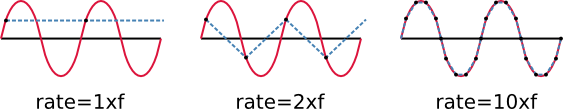
\includegraphics[width=\textwidth]{./img/samplerate}
\end{figure}
